\documentclass[conference]{IEEEtran}


%\usepackage{times}
 \usepackage{amsmath}
% \usepackage{subfig}
 \usepackage{amssymb}
 \usepackage{amsthm}
% \usepackage{color}
% \usepackage{amsbsy}
%  \usepackage{amstext}
%   \usepackage{amsopn}
%   \usepackage{amscd}
%     \usepackage{upref}
      \usepackage{graphicx}
\usepackage{subfig}
\usepackage{algorithm}
 \usepackage[noend]{algorithmic}
% \usepackage{url}
      \usepackage{cite}
\newcommand{\bE}{\mathbf{E}}
\newcommand{\bI}{\mathbf{I}}
\newcommand{\sfa}{\mathsf{a}}
\newcommand{\sfb}{\mathsf{b}}
\newtheorem{theorem}{Theorem}
\newtheorem{proposition}[theorem]{Proposition}
\newtheorem{lemma}[theorem]{Lemma}
\newtheorem{corollary}[theorem]{Corollary}
\newtheorem{defn}{Definition}



\long\def\symbolfootnote[#1]#2{\begingroup
\def\thefootnote{\fnsymbol{footnote}}\footnote[#1]{#2}\endgroup}




\title{Triple Fault-Tolerance Binary MDS Array Codes with Asymptotically Optimal Repair}



\begin{document}
\maketitle
\begin{abstract}
Binary maximal-distance separable (MDS) array code is one class of erasure codes, which is widely employed in distributed storage systems, due to its low computational complexity.
%with $k$ information columns and $r$ parity columns, of which each column storing $L$ bits such that any $k$ columns are sufficient to recover all the information bits.
%To reduce the probability of data unavailability, whenever a single disk fails, we need to recover the data in the failure disk.
%It is shown that if a single column fails, then we need to download at least $L/(d-k+1)$ bits in each of the $d$ surviving columns. The code is said to have the optimal repair property if the lowest bits downloaded is achieved.
%To reduce the probability of data unavailability, whenever a single column fails, we need to recover the data in the failure column. In the repair process of a single column failure, the amount of information transmitted from the surviving columns normalized by the storage size per column is termed repair bandwidth. It is shown that the repair bandwidth of an MDS erasure code that are constructed over a large enough finite field is lower bounded by $d/d-k+1$, where $d$ is the number of columns connected to repair the failure column.
%The existing MDS array codes, such as X-code, row-diagonal parity (RDP) code and EVENODD code can provide data availability with up to two disk failures. The optimal recovery algorithms of single disk failure for X-code, RDP and EVENODD are designed such that the recovery algorithms can reduce about 25\% of the information transmitted compared to the conventional recovery approach.
%We make several contributions. First,
However, one drawback of existing binary MDS array codes, such as RDP and X-code, is the high repair bandwidth.
In this paper, we present an explicit construction of triple fault-tolerance binary MDS array codes with asymptotically optimal repair bandwidth.

\end{abstract}




\section{Introduction}

Array codes are error-correcting codes with application to storage systems such as Redundant Arrays of Inexpensive Disks (RAID) architectures \cite{patterson1989introduction}. A binary array code consists of  arrays of size $L \times n$, with each element of an array storing one bit. We focus on binary array code, as its low computational complexity. Among the $n$ columns, $k$ \emph{information columns} store the information bits and $r=n-k$ \emph{parity columns} store the redundant bits. The $L$ bits in a column are stored in the same disk, or storage node. We refer to a disk as a column or a storage node interchangeably, and an entry in the array as a bit. When a storage node fails, the corresponding column of the array code is considered to be an \emph{erasure}. If the array code can tolerate any $r$ disk erasures, then it is called MDS array code. Examples of existing binary MDS array codes include X-code~\cite{xu1999x} and RDP~\cite{corbett2004row} with $r=2$, STAR \cite{huang2008star}, generalized RDP \cite{blaum2006family} and TIP \cite{Zhang2015TIP} can tolerate any three erasures.

When a disk fails in a distributed storage system, we will rebuild the erased bits in the failed disk by downloading some bits from the surviving disks. The amount of the downloaded bits in a repair process is called the \emph{repair bandwidth}. As the repair bandwidth plays a crucial role in the overall recovery time~\cite{corbett2004row} and influences the system service performance~\cite{holland1993fast}. It is important to minimize repair bandwidth.

The repair problem was first formulated and studied by Dimakis {\em et al.} in \cite{dimakis2010network}
using the concept of information flow graph. In the framework in~\cite{dimakis2010network}, a data file of size $B$ symbols is encoded and distributed to $n$ storage nodes, with each node storing $L$ symbols such that the file can be decoded from any $k$ of them. Furthermore, upon the failure of a storage node, a new node replaces the failed node by downloading $\beta$ symbols from each of $d$ surviving nodes, and the repair bandwidth is $d\beta$. It is shown in~\cite{dimakis2010network} that the optimal repair bandwidth is
\begin{equation}
\frac{(k+1)L}{2},
\label{optimal_repair}
\end{equation}
when $d=k+1$. Although the optimal repair bandwidth can be achieved in~\cite{tamo2013zigzag,agarwal2015alternate} over a large enough finite field, how to design binary MDS array codes to obtain the optimal repair bandwidth is less clear.


%It is challenging to repair a failed disk for binary MDS array codes with repair bandwidth as less as possible.
%A conventional approach is to download all the bits from each of the $k$ surviving disks and reconstruct the bits of the failure column, and the repair bandwidth is $k$ times of the number of bits in the failure disk.
It is shown in~\cite{xu2014single,xiang2010optimal} that the repair bandwidth of X-code and RDP is 50\% larger than the optimal value in \eqref{optimal_repair}.
For the case of two parity columns, butterfly code is proposed in~\cite{En2013Repair} with optimal repair. Wang \emph{et al.} \cite{Wang2013MDR,Wang2016Two} constructed the MDR codes over binary field and achieved the optimal repair. However, the optimal repair of binary MDS array codes with $r\geq 3$ parity columns is still an open problem.


In this paper, we give a new construction of binary MDS array codes with three parity columns. We show that the proposed binary MDS array code has comparable encoding complexity, compared to the existing binary MDS array codes. More importantly, the optimal repair bandwidth in (\ref{optimal_repair}) can be achieved asymptotically when $k$ is large enough, for any one information failure. 
The repair bandwidth reduction is made by a cyclic structure and a well-chosen encoding matrix, where the bits accessed in a repair intersect as much as possible. A ring with cyclic structure in reducing computational complexity in regenerating codes can be found in \cite{shumregenerating,Hou2016BASIC}. 
%But unlike the BR and BBV codes, arithmetic of polynomials modulo $x^p-1$ is used instead. Since in practice it is more likely to have single or double disk failures instead of five disk failures, we give an efficient method for repairing one and two disk failures. We also compare the encoding and repairing complexity of RDP, EVENODD, BBV code, Rabin-like code and the proposed array code.
%This enhances the fault-tolerant capability in compare with the RDP \cite{corbett2004row}, EVENODD \cite{blaum1995evenodd} and their variants in \cite{blaum2001evenodd,huang2008star,wang2012triple,blaum2006family}.
%The number of information columns of the proposed new MDS array code can be any positive integer from 2 to $p$.
%while the number of information of MDS array codes in \cite{corbett2004row,blaum1995evenodd,blaum2001evenodd,huang2008star,wang2012triple,tau2003efficient,blaum2006family,blaum1996mds} is restricted to be either $p-1$ or $p$.
%The new class of code yields a wider range of code parameters. of the proposed MDS array codes are also presented in this paper, which show that our MDS array codes have the advantage of lower computational complexity, compared to BBV code and Rabin-like code.
%Note that both our MDS array codes and binary cyclic codes \cite{shumregenerating} can be carried
%out by simple cyclic shift operations and binary additions. The MDS array codes focus on a specific encoding matrix. While the paper \cite{shumregenerating} proposed a framework of designing regenerating codes
%which employ XOR and bit-wise cyclic shifts.

%Another related work can be found in \cite{shumregenerating}, which proposes a framework of designing codes employing XOR and bit-wise cyclic shifts. In this paper, we focus on a specific encoding matrix.
This paper is organized as follows. We first give the construction of binary MDS array codes and then present the MDS property condition in Section~\ref{sec:constr}. In Section~\ref{sec:repair}, we give the repair algorithm for one single information erasure. 
%In Section~\ref{sec:com}, we compare the encoding complexity, decoding complexity and repair bandwidth with the existing binary MDS array codes.
We conclude in Section~\ref{sec:con}.


%We will show that any four nodes can reconstruct the data file in the next section.

\section{Binary MDS Array Codes}
\label{sec:constr}
In this section, we show how our proposed new binary MDS array codes are constructed.
\subsection{Construction of Binary MDS Array Codes}
Let $k\geq 3$ and $L=(p-1)\tau$ be positive integers, where $\tau=2^{k-2}$ and $p$ is a prime number such that $2^i\not\equiv 1\text{ mod } p$ for $i=1,2,\ldots,p-2$. Assume that a file of size $k(p-1)\tau$ denoted by information bits $s_{0,i},s_{1,i},\ldots, s_{(p-1)\tau-1,i}\in \mathbb{F}_2^{(p-1)\tau}$ for $i=1,2,\ldots,k$, which are employed to generate $3(p-1)\tau$ redundant bits $s_{0,j},s_{1,j},\ldots, s_{(p-1)\tau-1,j}\in \mathbb{F}_2^{(p-1)\tau}$ for $j=k+1,k+2,k+3$.
%The information bits $s_{0,i},s_{1,i},\ldots, s_{(p-1)\tau-1,i}$ are stored in the $i$ information column for $i=1,2,\ldots,k$, and the $(p-1)\tau$ redundant bits $s_{0,j},s_{1,j},\ldots, s_{L-1,j}$ are stored in the $j$ column (the $j-k$ parity or redundant column) for $j=k+1,k+2,k+3$.
For $\ell=1,2,\ldots,k+3$ and $\mu=0,1,\ldots,\tau-1$, we define the following short-hand notations
\begin{equation}
s_{(p-1)\tau+\mu,\ell} := \sum_{j=0}^{p-2} s_{j\tau+\mu,\ell}.
\label{eq:check1}
\end{equation}
We call $s_{(p-1)\tau+\mu,\ell}$ as the \emph{parity-check bit} associated with $s_{\mu,\ell},s_{\tau+\mu,\ell},\ldots,s_{(p-2)\tau+\mu,\ell}$. For example, when $p=3$, $k=4$ and $\tau=4$, we have the parity-check bit of $s_{0+\mu,\ell},s_{4+\mu,\ell}$ is $$s_{8+\mu,\ell}=s_{0+\mu,\ell}+s_{4+\mu,\ell}.$$ For $\ell=1,2,\ldots,k+3$, we present the bits $s_{0,\ell},s_{1,\ell},\ldots,s_{(p-1)\tau-1,\ell}$ in column $\ell$, together with $\tau$ parity-check bits $s_{(p-1)\tau,\ell},s_{(p-1)\tau+1,\ell},\ldots,s_{p\tau-1,\ell}$, by a polynomial $s_{\ell}(x)$ over the ring $\mathbb{F}_2[x]$,
$$s_\ell(x)=s_{0,\ell}+s_{1,\ell}x+s_{2,\ell}x^2+\ldots+s_{p\tau-1,\ell}x^{p\tau-1}.$$
The polynomial $s_{i}(x)$, corresponds to the $i$ information column for $i=1,2,\ldots,k$, is called \emph{data polynomial}. While the polynomial $s_{j}(x)$, corresponds to the $j-k$ parity column for $j=k+1,k+2,k+3$, is called \emph{coded polynomial}.


We write the $k$ data polynomials and $3$ coded polynomials as the row vector
\begin{equation}
[s_1(x),s_2(x),\cdots,s_{k+3}(x)],
\label{eq:data_clm}
\end{equation}
which can be computed by taking the product
\[
[s_1(x),s_2(x),\cdots,s_{k+3}(x)]= [s_1(x),s_2(x),\cdots,s_{k}(x)] \cdot \mathbf{G}
\]
with arithmetic performed in $\mathbb{F}_2[x]/(1+x^{p\tau})$,
where the $k\times (k+3)$ \emph{generator matrix} $\mathbf{G}$ is composed by the $k\times k$ identity matrix $\mathbf{I}$ and a $k\times 3$ \emph{encoding matrix} $\mathbf{P}$,
\[
\mathbf{P}:=
\begin{bmatrix}
 1&1&1 & \cdots & 1 &1\\
 x & x^{2} & x^{4}& \cdots & x^{2^{k-2}}&1\\
 1&x^{2^{k-2}}& x^{2^{k-3}}& \cdots & x^{2} & x \\
 \end{bmatrix}^T.
\label{matrixp}
\]
The proposed code is denoted as $\mathcal{C}(k,3,p)$. Note that we do not store the parity-check bits in the disk. It is present only for notational convenience. Consider an example of $k=4$ and $p=3$, the 32 information bits are represented by $s_{0,i}$, $s_{1,i}, \ldots, s_{7,i}$, for $i=1,2,3,4$. The encoding matrix of this example is
\begin{align*}
\begin{bmatrix}
1 & 1 & 1 & 1\\
x & x^2 & x^4 & 1 \\
1 & x^4 & x^2 & x
\end{bmatrix}^T.
\end{align*}
%The redundant bits stored in three parity columns of this example are computed and shown in Table \ref{t1}.
The example is illustrated in Fig.~\ref{example}, where the bit with bold type is parity-check bit.

\begin{figure}
\centering
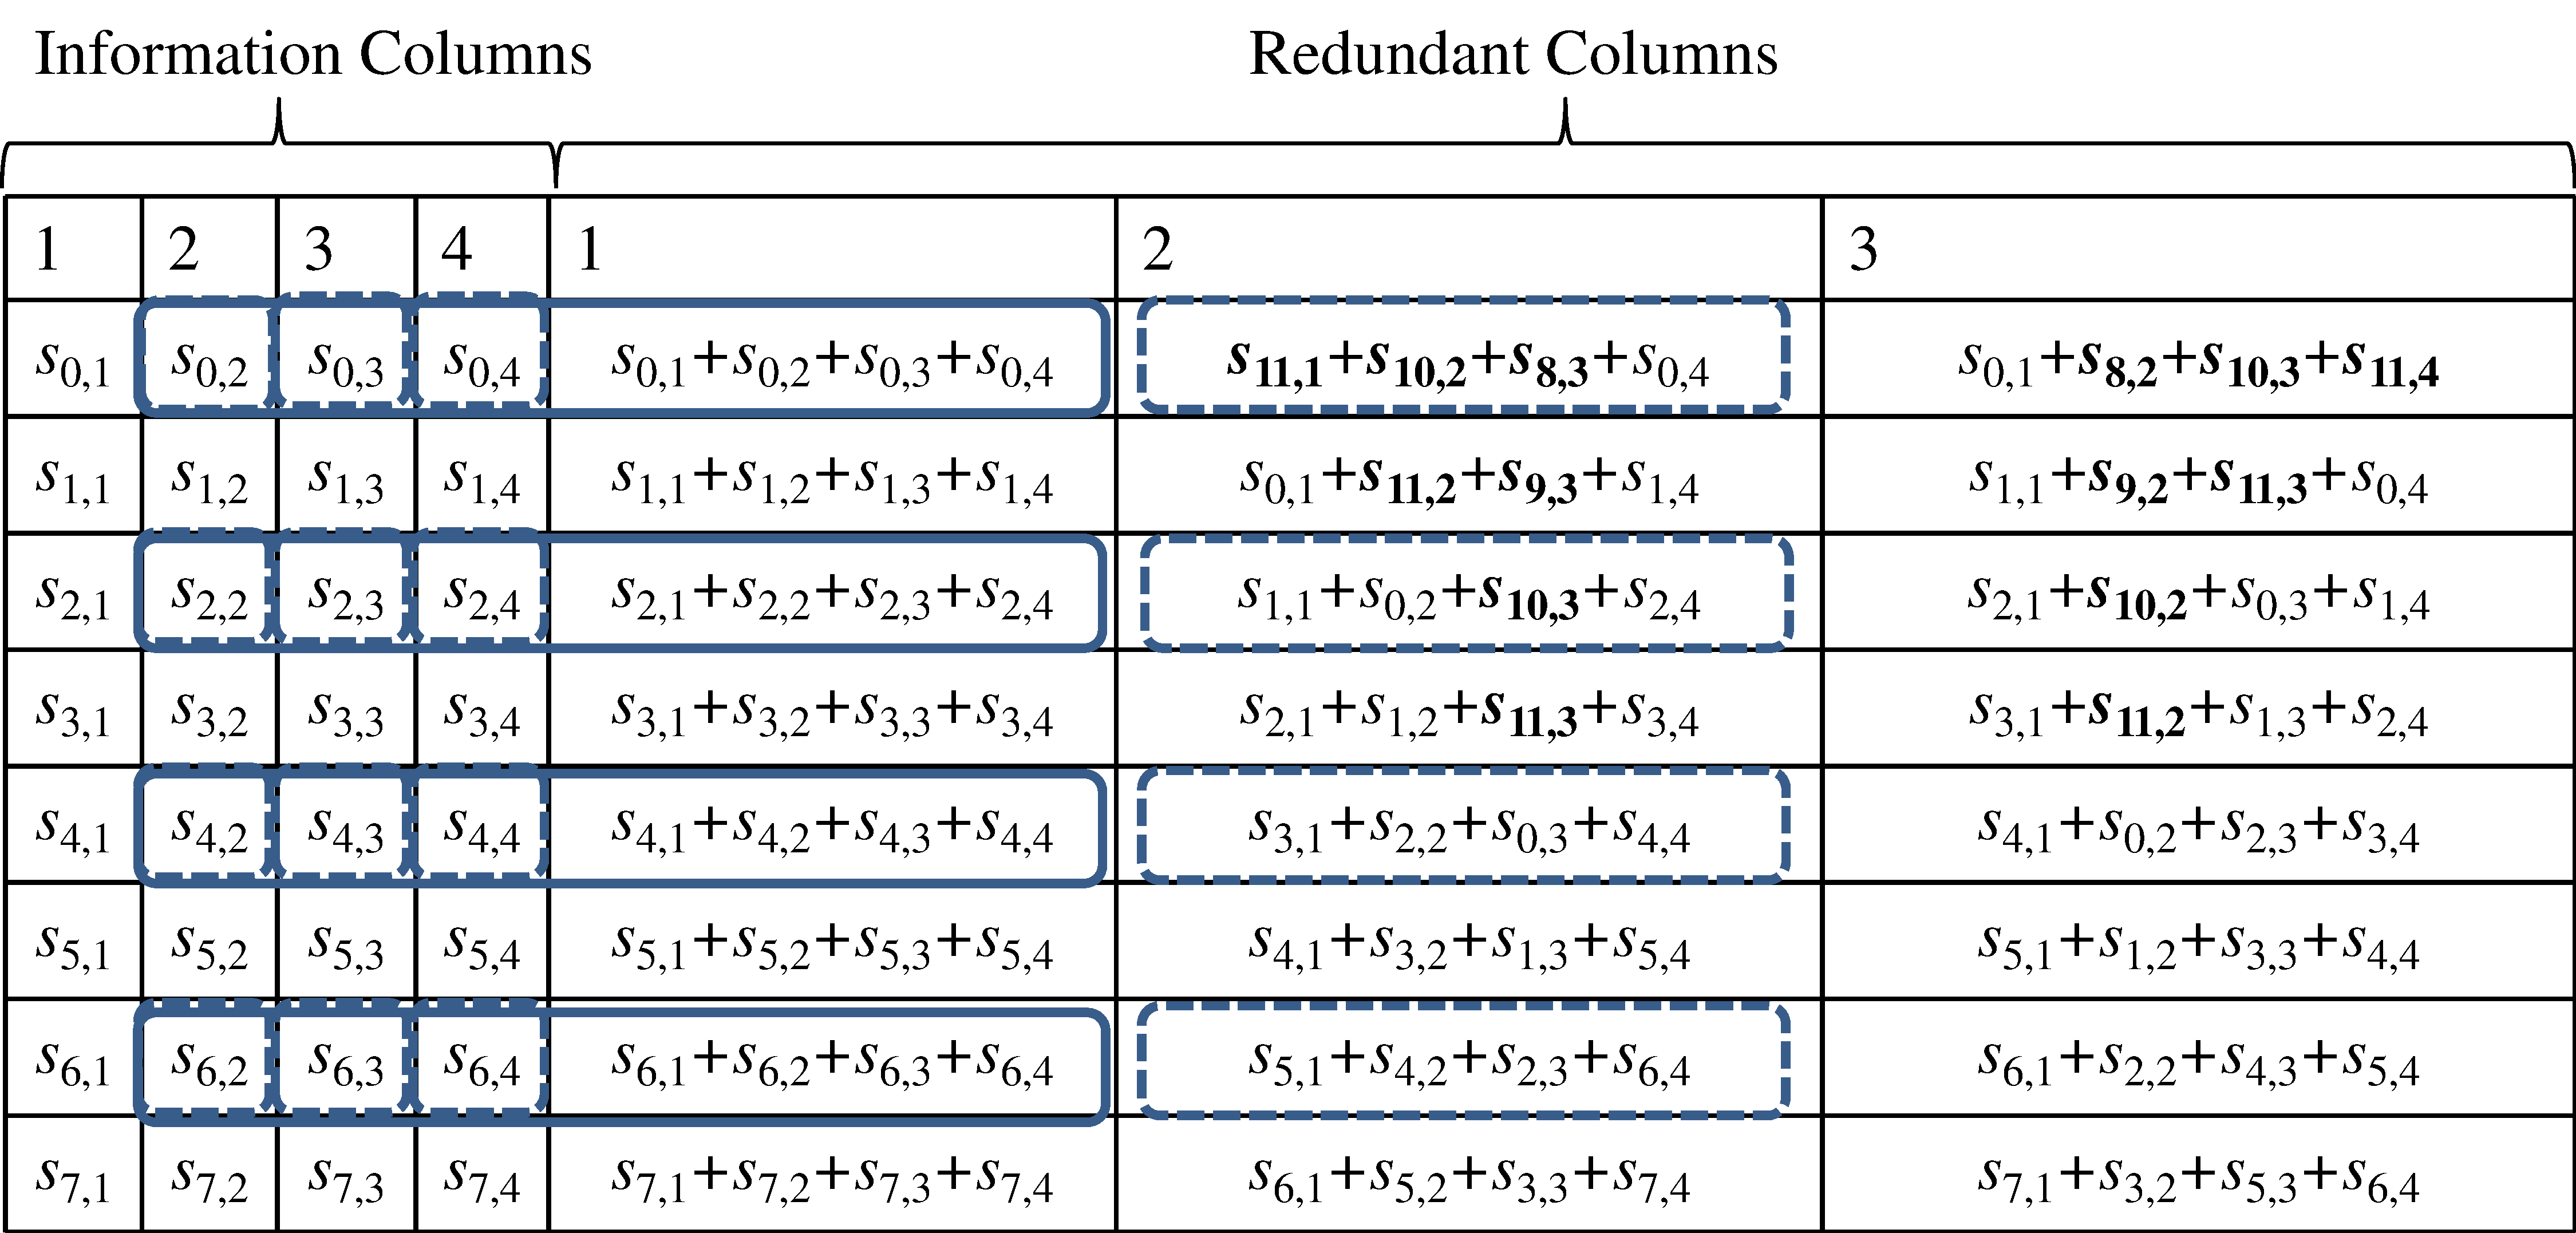
\includegraphics[width=0.5\textwidth]{example}
\caption{An example of storage code for three redundant columns. When information column 1 fails, the bits in the solid line box are downloaded to repair the information bits $s_{0,1},s_{2,1},s_{4,1},s_{6,1}$ and the bits in the dashed box are used to repair the information bits $s_{1,1},s_{3,1},s_{5,1},s_{7,1}$.}
\label{example}
\end{figure}




The encoding procedure can be described in terms of polynomials as follows. Given $k(p-1)\tau$ information bits, we append $\tau$ parity-check bits for each of $(p-1)\tau$ information bits and form the message vector $[s_1(x),s_2(x),\cdots,s_{k}(x)]$.
After obtaining the vector in \eqref{eq:data_clm},
 we store the coefficients of the terms in the polynomials of degrees 0 to $(p-1)\tau-1$.
The proposed array code can be considered as puncturing a systematic linear code over $\mathbb{F}_2[x]/(1+x^{p\tau})$.



\subsection{Proof of the MDS Property}
\label{sec:mds}
As we choose the prime $p$ such that the multiplication order of 2 mod $p$ is equal to $p-1$, we have $x^{p\tau}+1$ can be factorized as a product of two co-prime factors $x^{\tau}+1$ and
\[
M_p^{\tau}(x):=x^{(p-1)\tau}+x^{(p-2)\tau}+\cdots+x^{\tau}+1.
\]
By the Chinese Remainder Theorem, the ring $R_{p\tau}:=\mathbb{F}_{2}[x]/(x^{p\tau}+1)$ is isomorphic to the direct sum of $\mathbb{F}_2[x]/(x^{\tau}+1)$ and $\mathbb{F}_2[x]/(M_p^{\tau}(x))$. Indeed, we can set up an isomorphism
$$\theta: R_{p\tau} \rightarrow \mathbb{F}_2[x]/(x^{\tau}+1) \oplus \mathbb{F}_2[x]/(M_p^{\tau}(x))$$
by defining
\[
 \theta(f) := (f \bmod x^{\tau}+1, f \bmod M_p^{\tau}(x)).
\]
The mapping $\theta$ is a ring homomorphism and a bijection, because it has an inverse function $\phi(a,b)$  given by
\[
\phi(a,b) := a \cdot (x^{\tau}+1) + b \cdot e(x) \bmod x^{p\tau}+1,
\]
where $e(x) = x^{\tau} + x^{2\tau} + \cdots + x^{(p-1)\tau}$.
It can be checked that the composition $\phi \circ \theta$ is the identity map of~$R_{p\tau}$.

%As $x+1$ and $M_p^{\tau}(x)$ are irreducible polynomials in $\mathbb{F}_2[x]$, the rings $R_p$ is isomorphic to the direct sum of two finite fields $\mathbb{F}_2$ and $\mathbb{F}_{2^{p-1}}$.
By construction, $s_\ell(x)\equiv0\mbox{ mod }x^{\tau}+1$ for all $\ell=1,2,\ldots,k+3$. Hence, the first components of $\theta(s_\ell(x))$'s are all equal to zero. So, we are effectively working over the ring $\mathbb{F}_{2}[x]/(M_p^{\tau}(x))$. Recall that $\tau=2^{k-2}$, we have
\begin{align*}
M_p^{\tau}(x)=&x^{(p-1)\tau}+x^{(p-2)\tau}+\cdots+x^{\tau}+1 \\
=&(x^{p-1}+x^{p-2}+\cdots+x+1)^{\tau}:= (M_p(x))^{\tau}.
\end{align*}
As $M_p(x)$ is irreducible in $\mathbb{F}_2[x]$ \cite{Hou2016BASIC}, $\mathbb{F}_{2}[x]/(M_p^{\tau}(x))$ is isomorphic to the direct sum of $\tau$ finite fields $\mathbb{F}_2[x]/(M_p(x))$. With the same discussion in \cite{Hou2016BASIC}, we have the following result.


\begin{theorem}
$\mathcal{C}(k,3,p)$ is MDS if for $t=1,2,3$, the determinant of each $t\times t$ sub-matrix of $\mathbf{P}$ is not divisible by $x^p+1$.
  \label{thm:MDS2}
\end{theorem}
We need the following lemma in the proof of MDS property.
\begin{lemma}
Let $p$ be a prime such that the multiplicative order of 2 mod $p$ is equal to $p-1$. For $i=1,2,\ldots,p-2$, the following equation holds
\[
2^i+2^{i+\frac{p-1}{2}}\equiv 0 \text{ mod }p.
\]
\label{lemmap}
\end{lemma}
\begin{proof}
By Fermat's little theorem, we have $2^{p-1}\equiv 1\mod p$. As $2^{(p-1)/2}$ is a root of $x^2-1 \mod p$, so $2^{(p-1)/2}$ is equal to either $1 \text{ or } -1 \mod p$. Recall that the multiplicative order of 2 mod $p$ is equal to $p-1$, we have $2^{(p-1)/2}\not\equiv 1\mod p$ and $2^{(p-1)/2}+1\equiv 0\mod p$. Multiply both sides of the above equation by $2^i$ and we get the equation in Lemma \ref{lemmap} holds.
\end{proof}

The next theorem gives a sufficient MDS property condition.
\begin{theorem}
If $p \geq \max\{2k-8,k\}$ is a prime such that the multiplicative order of 2 mod $p$ is equal to $p-1$,  then the code $\mathcal{C}(k,3,p)$ satisfies the MDS property.
\label{thm:MDS5}
\end{theorem}
\begin{proof}
By Theorem~\ref{thm:MDS2}, we need to prove that for $t=1,2,3$, the determinant of each sub-matrix of $\mathbf{P}$ of size $t\times t$ is not divisible by $x^p+1$ in $\mathbb{F}_2[x]$.
When $t=1$, the determinant is equal to a power of $x$, and hence cannot be divisible by $x^p+1$. When $t=2$, the determinant can be classified as $x^i+1$ with $i=1,2$, $x^{2^i}+x^{2^j}$ with $0\leq i< j\leq k-2$, and $x^{2^i+2^{k-j-1}}+x^{2^j+2^{k-i-1}}$ with $1\leq i< j\leq k-2$.

It is easy to check that $x^i+1$ cannot be divisible by $x^p+1$ for $i=1,2$. If $x^{2^i}+x^{2^j}=x^{2^i}(1+x^{2^j-2^i})$ is divisible by $x^p+1$, then $2^j-2^i\equiv 0 \mbox{ mod } p$. We have $j\equiv i \mbox{ mod }p$, which contradicts the fact that $0\leq i< j<p$.
Suppose $x^{2^i+2^{k-j-1}}+x^{2^j+2^{k-i-1}}$ is divisible by $x^p+1$, we have
\[
2^j-2^i+2^{k-i-1}-2^{k-j-1}\equiv (2^{j-i}-1)(2^i+2^{k-j-1}) \equiv 0 \text{ mod }p.
\]
Since $p$ is a prime and $2^{j-i}-1 \not\equiv 0 \mbox{ mod } p$, this implies that $2^i+2^{k-j-1} \equiv 0 \mbox{ mod }p$.
By Lemma \ref{lemmap}, the equation $p=2k-2i-2j-1$ holds. As $1\leq i< j\leq k-2$, we have $p=2k-2i-2j-1\leq 2k-7$, which contradicts $p \geq 2k-8$.

For $t= 3$, we need to consider the following 3 determinants
\begin{equation}
\begin{vmatrix}
1 & 1 & 1 \\
x & x^{2^i} & 1 \\
1 & x^{2^{k-i-1}} & x \\
\end{vmatrix}
\label{deter1}
\end{equation}
with $1\leq i\leq k-2$,
\begin{equation}
\begin{vmatrix}
1 & 1 & 1 \\
x & x^{2^i} & x^{2^j} \\
1 & x^{2^{k-i-1}} & x^{2^{k-j-1}} \\
\end{vmatrix}
\label{deter2}
\end{equation}
with $1\leq i<j\leq k-2$, and
\begin{equation}
\begin{vmatrix}
1 & 1 & 1 \\
x^{2^i} & x^{2^j} & x^{2^{\ell}} \\
x^{2^{k-i-1}} & x^{2^{k-j-1}} & x^{2^{k-\ell-1}} \\
\end{vmatrix}
\label{deter3}
\end{equation}
with $1\leq i<j<\ell\leq k-2$.

%The determinant in (\ref{deter1}) is $x^{2^i+1}+x^{2^{k-i-1}+1}+x^{2^{k-i-1}}+x^{2^i}+x^2+1$,
If the determinant in (\ref{deter1}) is equal to zero in $\mathbb{F}_2[x]/(x^p+1)$, then the following six terms
$$
 x^{2^i+1},\ x^{2^{k-i-1}+1},\
 x^{2^{k-i-1}},\ x^{2^i},\
 x^{2} \text{ and } 1
$$
can be divided into 3 pairs such that the exponents in  each pair are congruent modulo~$p$. Consider the exponent of the last term. As $2^{k-i-1}$, $2^i$ and 2 are not congruent to 0 modulo~$p$, we only need to consider the case of 0 congruent to $2^i+1$ or $2^{k-i-1}+1$.
If 0 is congruent to $2^i+1$, then we have $i=\frac{p-1}{2}$ by Lemma \ref{lemmap} and the exponents of the remaining four terms $x^{2^{k-\frac{p-1}{2}-1}+1},\ x^{2^{k-\frac{p-1}{2}-1}},\ x^{p-1},\ x^{2}$ are not congruent modulo~$p$ with each other. If 0 is congruent to $2^{k-i-1}+1$, then we have $k-i-1=\frac{p-1}{2}$ by Lemma \ref{lemmap}, it indicates that
$$i=k-\frac{p+1}{2}<\frac{p-7}{2}-\frac{p+1}{2}=-4,$$
which contradicts the fact that $i\geq 1$.

The determinant in (\ref{deter2}) is
$$
(x^{2^i+2^{k-j-1}}+x^{2^j}+x^{2^{k-i-1}+1})+(x^{2^j+2^{k-i-1}}+x^{2^i}+x^{2^{k-j-1}+1}).
$$
None of the terms in the first parenthesis is equal to any term in the second parenthesis if the exponents are reduced modulo $p$, and \emph{vice versa}. Otherwise, we can deduce the contradiction of $1\leq i<j\leq k-2$.

Likewise, the determinant in (\ref{deter3}) can be re-arranged as
\begin{align*}
&(x^{2^j+2^{k-\ell-1}}+x^{2^{\ell}+2^{k-i-1}}+x^{2^{i}+2^{k-j-1}})+\\
&(x^{2^{\ell}+2^{k-j-1}}+x^{2^{i}+2^{k-\ell-1}}+x^{2^{j}+2^{k-i-1}}).
\end{align*}
None of the terms in the first parenthesis is equal to any term in the second parenthesis if the exponents are reduced modulo $p$, and \emph{vice versa}.
%Otherwise, we can deduce the contradiction of $1\leq i<j<\ell \leq k-2$.
This proves that the determinant in (\ref{deter3}) is not divisible by $x^p+1$, and completes the proof.

\end{proof}



\section{Asymptotically Optimal Repair of One Information Failure}
\label{sec:repair}

In this section, we always assume that information column $f$ erases, $f$ can be any value from 1 to $k$, we want to recover the bits $s_{0,f}$, $s_{1,f}, \ldots, s_{(p-1)\tau-1,f}$ stored in column $f$ by accessing bits from $k-1$ other information columns and 2 parity columns. Recall that we can compute the parity-check bits by \eqref{eq:check1}. For notational convenience, we refer the \emph{bits} of column $i$ as the $p\tau$ bits $s_{0,i}$, $s_{1,i}, \ldots, s_{p\tau-1,i}$.
Before giving the optimal repair algorithm, we formally define the \emph{parity set} as follows.
\begin{defn}
For $0\leq \ell \leq p\tau-1$, we define the $\ell$-th parity set of the first, the second and the third parity column as $$P_{\ell,1}=\{s_{\ell,1},s_{\ell,2},\ldots,s_{\ell,k}\},$$
$$P_{\ell,2}=\{s_{\ell-2^{0},1},s_{ \ell-2^{1},2},\ldots,s_{ \ell-2^{k-2},k-1},s_{\ell,k}\} \text{ and }$$
$$P_{\ell,3}=\{s_{\ell,1},s_{ \ell-2^{k-2},2},s_{ \ell-2^{k-3},3},\ldots,s_{ \ell-2^{0},k}\}$$ respectively.
\label{def1}
\end{defn}
Note that all the indices in Definition \ref{def1} and throughout the paper are taken modulo $p\tau$. From definition \ref{def1}, we see that the parity set $P_{\ell,j}$ consists of information bits which are used to generate the redundant bit $s_{\ell,k+j}$. When we say an information bit is repaired by a parity column, it means that we access the redundant bit of the parity column, and all the information bits in this parity set, except the erased bit.
Consider the example in Fig.~\ref{example}, suppose that the first column is erased. One can access the bits $s_{0,2},s_{0,3},s_{0,4}$ and the redundant bit $s_{0,1}+s_{0,2}+s_{0,3}+s_{0,4}$ to rebuild $s_{0,1}$ by
$$s_{0,2}+s_{0,3}+s_{0,4}+(s_{0,1}+s_{0,2}+s_{0,3}+s_{0,4}).$$

%During the repair process, one bit is said to be repaired by $i$-th parity, if we use the XOR-ing of its parity set in order to compute its value. This can be done by simply accessing and reading in the chosen columns the values of the rest of the intermediates. Each of the erasure information bits can be recovered from a parity of the three parity columns.
%, each erased bit can be computed either by using the first parity or by $\lceil \frac{2i}{k}\rceil+1$-th parity set.
%$\lceil \frac{2i}{k}\rceil+1$-Th.


\begin{algorithm}
\begin{algorithmic}[1]
\STATE {Suppose the information column $f$ is failed.}
    \IF {$f\in\{1, 2,\ldots, \lceil k/2 \rceil\}$.}
            \STATE {Repair the bit $s_{\ell,f}$ by the first parity, for $\ell \mod 2^f \in \{0,1,2,\ldots,2^{f-1}-1\}$. Otherwise, repair the bit $s_{\ell,f}$ by the second parity, for $\ell \mod 2^f \in \{2^{f-1},2^{f-1}+1,2^{f-1}+2,\ldots,2^{f}-1\}$.}
    \ENDIF
     \IF {$f\in\{\lceil k/2 \rceil+1, \lceil k/2 \rceil+2,\ldots, k\}$.}
            \STATE {Repair the bit $s_{\ell,f}$ by the first parity, for $\ell \mod 2^f \in \{0,1,2,\ldots,2^{f-1}-1\}$. Otherwise, repair the bit $s_{\ell,f}$ by the third parity, for $\ell \mod 2^f \in \{2^{f-1},2^{f-1}+1,2^{f-1}+2,\ldots,2^{f}-1\}$.}
    \ENDIF
    \caption{Repair of one information failure}
    \label{alg:A1}
\end{algorithmic}
\end{algorithm}

The repair algorithm is stated in Algorithm~\ref{alg:A1}.
Let's consider the example in Fig.~\ref{example} to illustrate the repair process more understandable. In the example, $k=5$, $d=5$ and $\tau=4$.
%If a single information column is erased, we will rebuild each information bit in the erased column either by downloading some bits in the surviving columns.
%In particular, we access the parity bit, and all the information bits in this set, except the erased bit.
Suppose that the first information column fails, i.e., $f=1$. By steps 2 and 3 in Algorithm~\ref{alg:A1}, we can repair the bits $s_{\ell,1}$ by the first parity column for $\ell \equiv 0 \mod 2$ and $0\leq \ell\leq 7$. More specifically, the bits $s_{0,1},s_{2,1},s_{4,1},s_{6,1}$ are rebuilt by
\begin{align*}
& s_{0,1}=s_{0,2}+s_{0,3}+s_{0,4}+(s_{0,1}+s_{0,2}+s_{0,3}+s_{0,4}) \\
& s_{2,1}=s_{2,2}+s_{2,3}+s_{2,4}+(s_{2,1}+s_{2,2}+s_{2,3}+s_{2,4}) \\
& s_{4,1}=s_{4,2}+s_{4,3}+s_{4,4}+(s_{4,1}+s_{4,2}+s_{4,3}+s_{4,4}) \\
& s_{6,1}=s_{6,2}+s_{6,3}+s_{6,4}+(s_{6,1}+s_{6,2}+s_{6,3}+s_{6,4}).
\end{align*}
As $f=1\in\{1,2\}$, the other information bits $s_{\ell,1}$ is repaired by the second parity column for $\ell \equiv 1 \mod 2$ and $0\leq \ell\leq 7$. Therefor, the bits $s_{1,1},s_{3,1},s_{5,1},s_{7,1}$ are rebuilt by
\begin{align*}
s_{1,1}=s_{0,2}+s_{10,3}+s_{2,4}+&(s_{1,1}+s_{0,2}+s_{10,3}+s_{2,4}) \\
s_{3,1}=s_{2,2}+s_{0,3}+s_{4,4}+&(s_{3,1}+s_{2,2}+s_{0,3}+s_{4,4}) \\
s_{5,1}=s_{4,2}+s_{2,3}+s_{6,4}+&(s_{5,1}+s_{4,2}+s_{2,3}+s_{6,4}) \\
s_{7,1}=s_{6,2}+s_{4,3}+s_{8,4}+&(s_{11,1}+s_{10,2}+s_{8,3}+s_{0,4})\\
+&(s_{3,1}+s_{2,2}+s_{0,3}+s_{4,4}).
\end{align*}
As we can compute $s_{10,3}$ by $s_{6,3}+s_{2,3}$ and $s_{8,4}$ by $s_{4,4}+s_{0,4}$, so we do not need to download the bits $s_{10,3}$ and $s_{8,4}$.
Therefore, we count that we need to download 4 bits from each of the three information columns and two parity columns. There are total 20 bits downloaded from 5 columns to repair the bits of the first information column.
Namely, only half of the bits of the helping columns are accessed. In Fig.~\ref{example}, the bits in the solid line box are downloaded to repair the information bits $s_{0,1},s_{2,1},s_{4,1},s_{6,1}$ and the bits in the dashed box are used to repair the information bits $s_{1,1},s_{3,1},s_{5,1},s_{7,1}$.

Suppose node 2 fails, i.e,. $f=2$. By steps 2 and 3 in Algorithm~\ref{alg:A1}, we can repair the bits $s_{0,2},s_{1,2},s_{4,2},s_{5,2}$ by
\begin{align*}
& s_{0,2}=s_{0,1}+s_{0,3}+s_{0,4}+(s_{0,1}+s_{0,2}+s_{0,3}+s_{0,4}) \\
& s_{1,2}=s_{1,1}+s_{1,3}+s_{1,4}+(s_{1,1}+s_{1,2}+s_{1,3}+s_{1,4}) \\
& s_{4,2}=s_{4,1}+s_{4,3}+s_{4,4}+(s_{4,1}+s_{4,2}+s_{4,3}+s_{4,4}) \\
& s_{5,2}=s_{5,1}+s_{5,3}+s_{5,4}+(s_{5,1}+s_{5,2}+s_{5,3}+s_{5,4}).
\end{align*}
By steps 2 and 3, we should repair the bits $s_{2,2},s_{3,2},s_{6,2},s_{7,2}$ by
\begin{align*}
s_{2,2}&=s_{3,1}+s_{0,3}+s_{4,4}+(s_{3,1}+s_{2,2}+s_{0,3}+s_{4,4}) \\
s_{3,2}&=s_{4,1}+s_{1,3}+s_{5,4}+(s_{4,1}+s_{3,2}+s_{1,3}+s_{5,4}) \\
s_{6,2}&=s_{7,1}+s_{4,3}+s_{0,4}+s_{4,4}+\\
&(s_{11,1}+s_{10,2}+s_{8,3}+s_{0,4})+(s_{3,1}+s_{2,2}+s_{0,3}+s_{4,4}) \\
s_{7,2}&=s_{0,1}+s_{4,1}+s_{5,3}+s_{1,4}+s_{5,4}+\\
&(s_{0,1}+s_{11,2}+s_{9,3}+s_{1,4})+(s_{4,1}+s_{3,2}+s_{1,3}+s_{5,4}).
\end{align*}
As a result, the 8 bits stored in the second information column can be recovered by downloading 6 bits from the first information column and 4 bits from each of the third information column, the fourth information column, the first parity column and the second parity column. There are total 22 bits downloaded in the repair process. It can be verified that for the code in Fig.~\ref{example}, the third information column and the last information column can be rebuilt by accessing 22 bits and 20 bits from 5 columns respectively.


\begin{theorem}
When $f\in\{1, 2,\ldots, \lceil k/2 \rceil\}$, the repair bandwidth of information column $f$ by Algorithm \ref{alg:A1} is
\begin{align*}
(p-1)((k+2)2^{k-3}-2^{k-f-2}).
\end{align*}
\label{thmrep}
\end{theorem}
\begin{proof}
By Algorithm \ref{alg:A1}, the bits $s_{\ell,f}$ are repaired by the parity sets $P_{\ell,1}$ of the first parity column for $\ell \mod 2^f \in \{0,1,2,\ldots,2^{f-1}-1\}$ and $\ell < (p-1)\tau$. Therefore, we need to access $(p-1)\tau/2$ information bits $s_{\ell,i}$ from each of the remaining $k-1$ information columns for $i\in\{1,2,\ldots,f-1,f+1,\ldots,k\}$ and $\ell \mod 2^f \in \{0,1,2,\ldots,2^{f-1}-1\}$, and download $(p-1)\tau/2$ redundant bits $s_{\ell,k+1}$ for $\ell \mod 2^i \in \{0,1,2,\ldots,2^{i-1}-1\}$ from the first parity column. Thus, there are $k(p-1)\tau/2$
bits to be downloaded.

For $\ell \mod 2^f \in \{2^{f-1},2^{f-1}+1,2^{f-1}+2,\ldots,2^{f}-1\}$, the bits $s_{\ell,f}$ are repaired by $P_{\ell+2^{f-1},2}$. Recall that
$$P_{\ell+2^{f-1},2}=\{s_{\ell+2^{f-1}-2^{0},1},\ldots,s_{\ell+2^{f-1}-2^{k-2},k-1},s_{\ell+2^{f-1},k}\}.$$
So we need to access $(p-1)\tau/2$ redundant bits $s_{\ell+2^{f-1},k+2}$. For column $i$ with $i\in\{1,2,\ldots,f-1\}$, we need $(p-1)\tau/2$ bits $s_{\ell,i}$ for all the values of $\ell \mod 2^f$ in the set
$$\{0,1, \ldots, 2^{f-1}-2^{i-1}-1,2^{f}-2^{i-1},2^{f}-2^{i-1}+1,\ldots,2^{f}-1\}.$$
While for column $i$ with $i\in\{f+1,f+2,\ldots,k\}$, we need $(p-1)\tau/2$ bits $s_{\ell,i}$ for $\ell \mod 2^f \in \{0,1,2,\ldots,2^{f-1}-1\}$.

Note that the bits $s_{\ell,i}$ for $\ell \mod 2^f \in \{0,1,2,\ldots,2^{f-1}-1\}$ and $\ell < (p-1)\tau$ have downloaded in the repair by the first parity column. Thus, we only need to download $(p-1)\tau/2$ redundant bits from the second parity column, and
$(p-1)2^{k+i-f-3}$
bits from column $i$ for $i=1,2,\ldots,f-1$.

We can count that the total number of bits downloaded from $k+2$ columns to repair the information column $f$ is
\begin{align*}
&\underbrace{k(p-1)2^{k-3}}_{\text{the first parity column}}+\underbrace{\sum_{i=1}^{f-1}(p-1)2^{k+i-f-3}}_{\text{the second parity column}}\\
&=(p-1)((k+2)2^{k-3}-2^{k-f-2}).
\end{align*}
\end{proof}
When $1\leq f\leq \lceil k/2 \rceil$, the repair bandwidth of column $k+1-f$ is the same of that of column $f$ according to Algorithm~\ref{alg:A1}. Therefore, we only consider the cases of $1\leq f\leq \lceil k/2 \rceil$.
By Theorem~\ref{thmrep}, repair bandwidth increases with $f$ increases.
When $f=1$, the repair bandwidth is $(k+1)(p-1)2^{k-3}$, which achieves the optimal value in \eqref{optimal_repair}. Even for the worst case of $f=\lceil k/2\rceil$, the repair bandwidth is
\begin{align*}
(p-1)((k+2)2^{k-3}-2^{k-\lceil k/2\rceil-2})< (p-1)(k+2)2^{k-3},
\end{align*}
which is strictly less than $\frac{k+2}{k+1}$ times of the value in \eqref{optimal_repair}. Therefore, the repair bandwidth of any one information failure can achieve the optimal repair in \eqref{optimal_repair} asymptotically when $k$ is large enough.

It should be noted that the parity sets of the first parity column in our codes are the same of that of the first parity column in RDP and EVENODD. The key difference of our codes and the existing binary MDS array codes is the construction of the second and the third parity columns. First, the parity sets of the second and the third parity columns in our codes are not bits that correspond to straight lines in the array, but the bits that correspond to polygonal lines. Second, the row number of the array in our codes is divisible by $2^{k-2}$. The two properties are essential for reducing the repair bandwidth.




%Let $a, b$ be integers between 1 and $k$.
%Suppose that columns $a$ and $b$ are erased. We want to recover the lost information bits in columns $a$ and $b$ by reading columns $i$, for $i\in\{1,2,\ldots, k\}\setminus\{a,b\}$, and the first two parity columns.
%
%The accessed bits are represented by polynomials
%$s_i(x)$,
%\[ s_{k+1}(x) = \sum_{i=1}^{k}s_{i}(x) \text{ and } s_{k+2}(x) = s_{k}(x)+\sum_{i=1}^{k-1}s_{i}(x)x^{2^{i-1}}.
%\]
%Let $f_1(x)$ and $f_2(x)$ be the polynomials by subtracting
%the known values of $s_i(x)$,  for  $i \in\{1,2,\ldots, k\}\setminus\{a,b\}$, from $s_{k+1}(x)$ and $s_{k+2}(x)$, respectively. Without loss of generality, we assume that $1<a<b<k$. As the decoding method of the other cases is analogous. The two erasures can be repaired by solving the following system of linear equations
%\[
%\begin{bmatrix}
%1 & 1 \\
%x^{2^{a-1}} & x^{2^{b-1}}
%\end{bmatrix}
%\begin{bmatrix}
% s_{a}(x) \\ s_{b}(x)
%\end{bmatrix}
%=
%\begin{bmatrix}
%f_1(x) \\ f_2(x)
%\end{bmatrix}.
%\]
%Therefore we can solve for $s_a(x)$ by
%$(x^{2^{a-1}} + x^{2^{b-1}})^{-1}(x^{2^{b-1}}f_1(x)+f_2(x))$,
%and $s_{b}(x)$ by $s_a(x)+f_1(x)$.
%
%
%
%Note that $x^{i}f_1(x) + x^{j}f_2(x)$ can be computed by cyclically shifting $f_1(x)$ and $f_2(x)$ to the right by $i$ and $j$, respectively, and adding the resulting polynomials.
%%Multiplication by $x^{i+j}$ is simply cyclically shifting to the right by $i+j$.
%Before giving the decoding complexity, we need the following lemma about how to compute the division of the form $1/(1+x^b)$ in $R_{p\tau}$.
%\begin{lemma}
%Given the equation $(1+x^b)s(x)=c(x)$, where $b$ is a positive integer and $s(x),c(x)\in \mathbb{F}_2[x]/M_p^{\tau}(x)$. Let $(b,\tau)=a$, we have the following equation
%%can represent a coefficient $s_{(p-1)b\frac{\tau}{a}}$ of $s(x)$ as
%$$s_{(p-1)b\tau/a}=\sum_{i=1}^{\tau/a}c_{bi}+\sum_{i=2\tau/a+1}^{3\tau/a}c_{bi}+\cdots+\sum_{i=(p-3)\tau/a+1}^{(p-2)\tau/a}c_{bi},$$
%where $s(x)=\sum_{i=0}^{p\tau-1}s_ix^i$ and $c(x)=\sum_{i=0}^{p\tau-1}c_ix^i$.
%\label{lm:inverse}
%\end{lemma}
%\begin{proof}
%By the equation $(1+x^b)s(x)=c(x)$, we have,
%\begin{align*}
%c_{b(\ell\frac{\tau}{a}+1)}+c_{b(\ell\frac{\tau}{a}+2)}+\cdots+c_{b(\ell+1)\frac{\tau}{a}}
%=s_{b\ell\frac{\tau}{a}}+s_{b(\ell+1)\frac{\tau}{a}}.
%\end{align*}
%We thus have that
%\begin{align*}
%&\sum_{i=1}^{\tau/a}c_{bi}+\sum_{i=2\tau/a+1}^{3\tau/a}c_{bi}+\cdots+\sum_{i=(p-3)\tau/a+1}^{(p-2)\tau/a}c_{bi}+s_{(p-1)b\tau/a}\\
%=&s_0+s_{b\tau/a}+s_{2b\tau/a}+\cdots+s_{(p-2)b\tau/a}+s_{(p-1)b\tau/a}\\
%=&s_0+s_{\tau}+s_{2\tau}+\cdots+s_{(p-2)\tau}+s_{(p-1)\tau}=0.
%\end{align*}
%%In the equations above, the indices are taken modulo $p\tau$.
%The second equality follows from the fact that $\ell b\tau/a \neq 0 \mod p\tau$ for $(b/a,p)=1$ and $1\leq \ell \leq p-1$.
%\end{proof}
%By the same argument of Lemma~\ref{lm:inverse}, we have that
%$$s_{(p-1)b\frac{\tau}{a}+j}=\sum_{i=1}^{\tau/a}c_{bi+j}+\sum_{i=2\frac{\tau}{a}+1}^{3\tau/a}c_{bi+j}+\cdots+\sum_{i=(p-3)\frac{\tau}{a}+1}^{(p-2)\tau/a}c_{bi+j},$$
%for $1\leq j\leq a$.
%All the other coefficients of $s(x)$ can be computed recursively by
%$$c_{(p-1)b\tau/a+\ell}=s_{(p-1)b\tau/a-b+\ell}+s_{(p-1)b\tau/a+\ell}$$
%for $\ell=1,2,\ldots,p\tau-1$. There are at most $\frac{3p\tau}{2}$ XORs involved in the solving $s(x)$ from $(1+x^b)s(x)=c(x)$.





%Consider the decoding process. Adding the parity-check bits to formulate $k-2$ data polynomials and 2 coded polynomials takes $k\tau(p-2)$ XORs. Computing the polynomials $f_1(x)$ and $f_2(x)$ involves $2(k-2)p\tau$ XORs.
%In the last step, recover $s_a(x)$ and $s_b(x)$ takes $3.5p\tau$ XORs at most by Lemma~\ref{lm:inverse}.
%Thus, the decoding complexity of two information erasures is
%\[
%\frac{k\tau(p-2)+2(k-2)p\tau+3.5p\tau}{k(p-1)\tau}<3+1/(p-1)+3.5/k.
%\]




%As there is no explicite decoding algorithm for Gad's code and MDR code, we don't give the decoding complexity in Table \ref{table:A}.


\section{Conclusion}
\label{sec:con}
In this paper, we present new binary MDS array codes with three parity columns such that the repair bandwidth of one information column is asymptotically optimal. 

We define the encoding complexity as the average number of XORs needed to generate one redundant bit. By the construction, we should first compute $k\tau$ parity-check bits by \eqref{eq:check1}, which involves $k\tau(p-2)$ XORs. Then generate the coefficients of degree from 0 to $(p-1)\tau-1$ for three coded polynomials that take $3(p-1)\tau(k-1)$ XORs. Therefore, the encoding complexity is
\[
\frac{k\tau(p-2)+3(p-1)\tau(k-1)}{3(p-1)\tau}<4k/3-1,
\]
which is comparable to the encoding complexity of the existing binary MDS array codes.

%If there are two information failures, we may decode the two failures with low computational complexity. First, we may download all the bits in the other $k-2$ information columns and any two parity columns, formulate the corresponding data polynomials and coded polynomials, subtract all the data polynomials from the two coded polynomials. Then, we can recover one information bit with a method similar to Lemma 13 in \cite{Hou2016BASIC}, and recover all the other information bits recursively. When there are three information failures, we may download all the other bits and decode the failure data polynomials by Cramer's rule.

The future work includes the extension of the construction with more parity columns and efficient repair algorithm for parity column.



\appendices

\bibliographystyle{IEEEtran}

\bibliography{CNC}

\end{document}


